\documentclass[letterpaper,12pt]{article}
\usepackage{fullpage}
\usepackage{fancyvrb,fancyhdr}
\usepackage{amsfonts}
\usepackage{array}
\usepackage{multirow}
\usepackage{amsmath, amssymb, amsthm}
\usepackage{graphicx,longtable, booktabs}
\usepackage[flushleft]{threeparttable}
\usepackage[footnotesize,center]{subfigure}
\usepackage{enumerate}
\usepackage{lastpage}
\usepackage{url}
\usepackage{mathrsfs}
\usepackage{cancel}
\usepackage{cite}
\usepackage{soul}
\usepackage{MnSymbol}
% Pseudo Code
\usepackage{algorithm}
\usepackage{algorithmic}
% Comments are in red
\usepackage{color}

\oddsidemargin 0in \evensidemargin 0in
\topmargin -0.5in \headheight 0.25in \headsep 0.25in
\textwidth 6.5in \textheight 9in %\marginparsep 0pt \marginparwidth 0pt
\parskip 0ex \parindent 10pt \footskip 20pt

\newfont{\bssten}{cmssbx10}
\newfont{\bssnine}{cmssbx10 scaled 900}
\newfont{\bssdoz}{cmssbx10 scaled 1200}

\pagestyle{fancy}
\fancyhead[LO]{\bssnine Diabetic Retinopathy}
% \fancyhead[R]{} \fancyhead[LO]{}
\fancyhead[RO]{\bssnine \thepage/\pageref{LastPage}}
%\fancyhead[RO]{\thepage}
\lfoot{} \cfoot{} \rfoot{}

%\usepackage[pdftex]{hyperref}

\def\t#1{{\tt #1}}
\newfont{\sserifn}{cmssbx10 at 11pt}
\newfont{\sserifo}{cmssbx10 at 12pt}

% Defining new \vect{} command to use a bold letter as a vector
\newcommand{\vect}[1]{\mathbf{#1}}
\newcommand{\erfc}{\mathrm{erfc}}
\newcommand{\figref}[1]{Figure~\ref{#1}}
\newcommand{\tableref}[1]{Table~\ref{#1}}
\newcommand{\eqsref}[1]{Eq.~\ref{#1}}
\newcommand{\algref}[1]{Algorithm~\ref{#1}}

%opening                    

\usepackage[para,multiple]{footmisc}
\newcommand{\jose}[1]{\comment{red}{#1}}
\newcommand{\imagej}{ImageJ }

\title{Convolution Neural Network Approach to Diagnosing Diabetic Retinopathy}
\author{Jos\'e Solomon \thanks{jose.e.solomon@gmail.com} } 

\date{}
\begin{document}

\maketitle
\begin{abstract}
This is the first draft of the project report of the diabetic retinopathy diagnosis using convolution neural networks (ConvNN). It is derived from the Kaggle Diabetic Retinopathy \cite{kaggle} aimed at creating a robust algorithm to automate the process of classifying the level of diabetic retinopathy found in retinal scans. the purpose of this initial draft is primarily to describe how the ConvNN work, and the inter-dependencies  of its various functional elements. In the final draft, details of the implementation will be given and various resulting performance metrics will be reviewed.
\end{abstract}
\tableofcontents

\section{Introduction}

There are two key facets to the project: first is the concept of the diabetic retinopathy and it's diagnosis; the second is ConvNN and it general functional principles as applied to digital imaging processing and categorization. We begin with a cursory description of the former, and then focus the bulk of the theoretical discussion on the latter.

\section{Diabetic Retinopathy}

Diabetic retinopathy (DR) is a disease that generally afflicts those who have dealt with diabetes for a period of 5 years or more \cite{nih}. It is defined specifically as the deterioration of blood vessels that feed the retina of the human eye, as illustrated in \figref{eye} below.
\begin{figure}[htbp]
\begin{center}
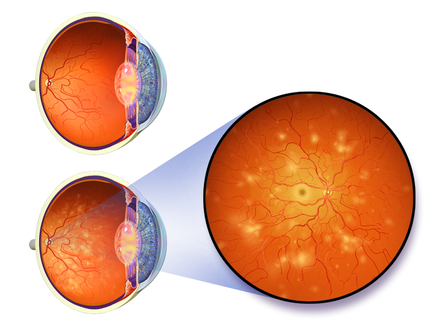
\includegraphics[scale=0.6]{images/illustration.png}
\caption{Diabetic retinopathy in comparison to a normal eye \cite{wiki}}
\label{eye}
\end{center}
\end{figure}
The primary cause of DR is that as a byproduct of the condition of diabetes, thinner blood vessels in the human body tend to form abnormal branching structures and thinning walls. This leads to either deteriorated blood supply to the effected areas or actual hemorrhaging. In terms of the retina, this leads to blind spots forming in the field of vision of the afflicted individual. 
To diagnose the condition, a retinal scan of the eye is taken and a classification is assigned depending on the number of abnormal vein branching, wall thickness of the blood vessels and blood stains observed. DR is categorized on a scale from 0 to 4, and examples of level 0 and 4 DR are given below. It should be noted that this method of categorizing DR is not fundamentally rigorous in nature and is more of a qualitative scale. 

\begin{figure}[htbp]
\begin{center}
 \subfigure[Level 0 DR]{\label{reference}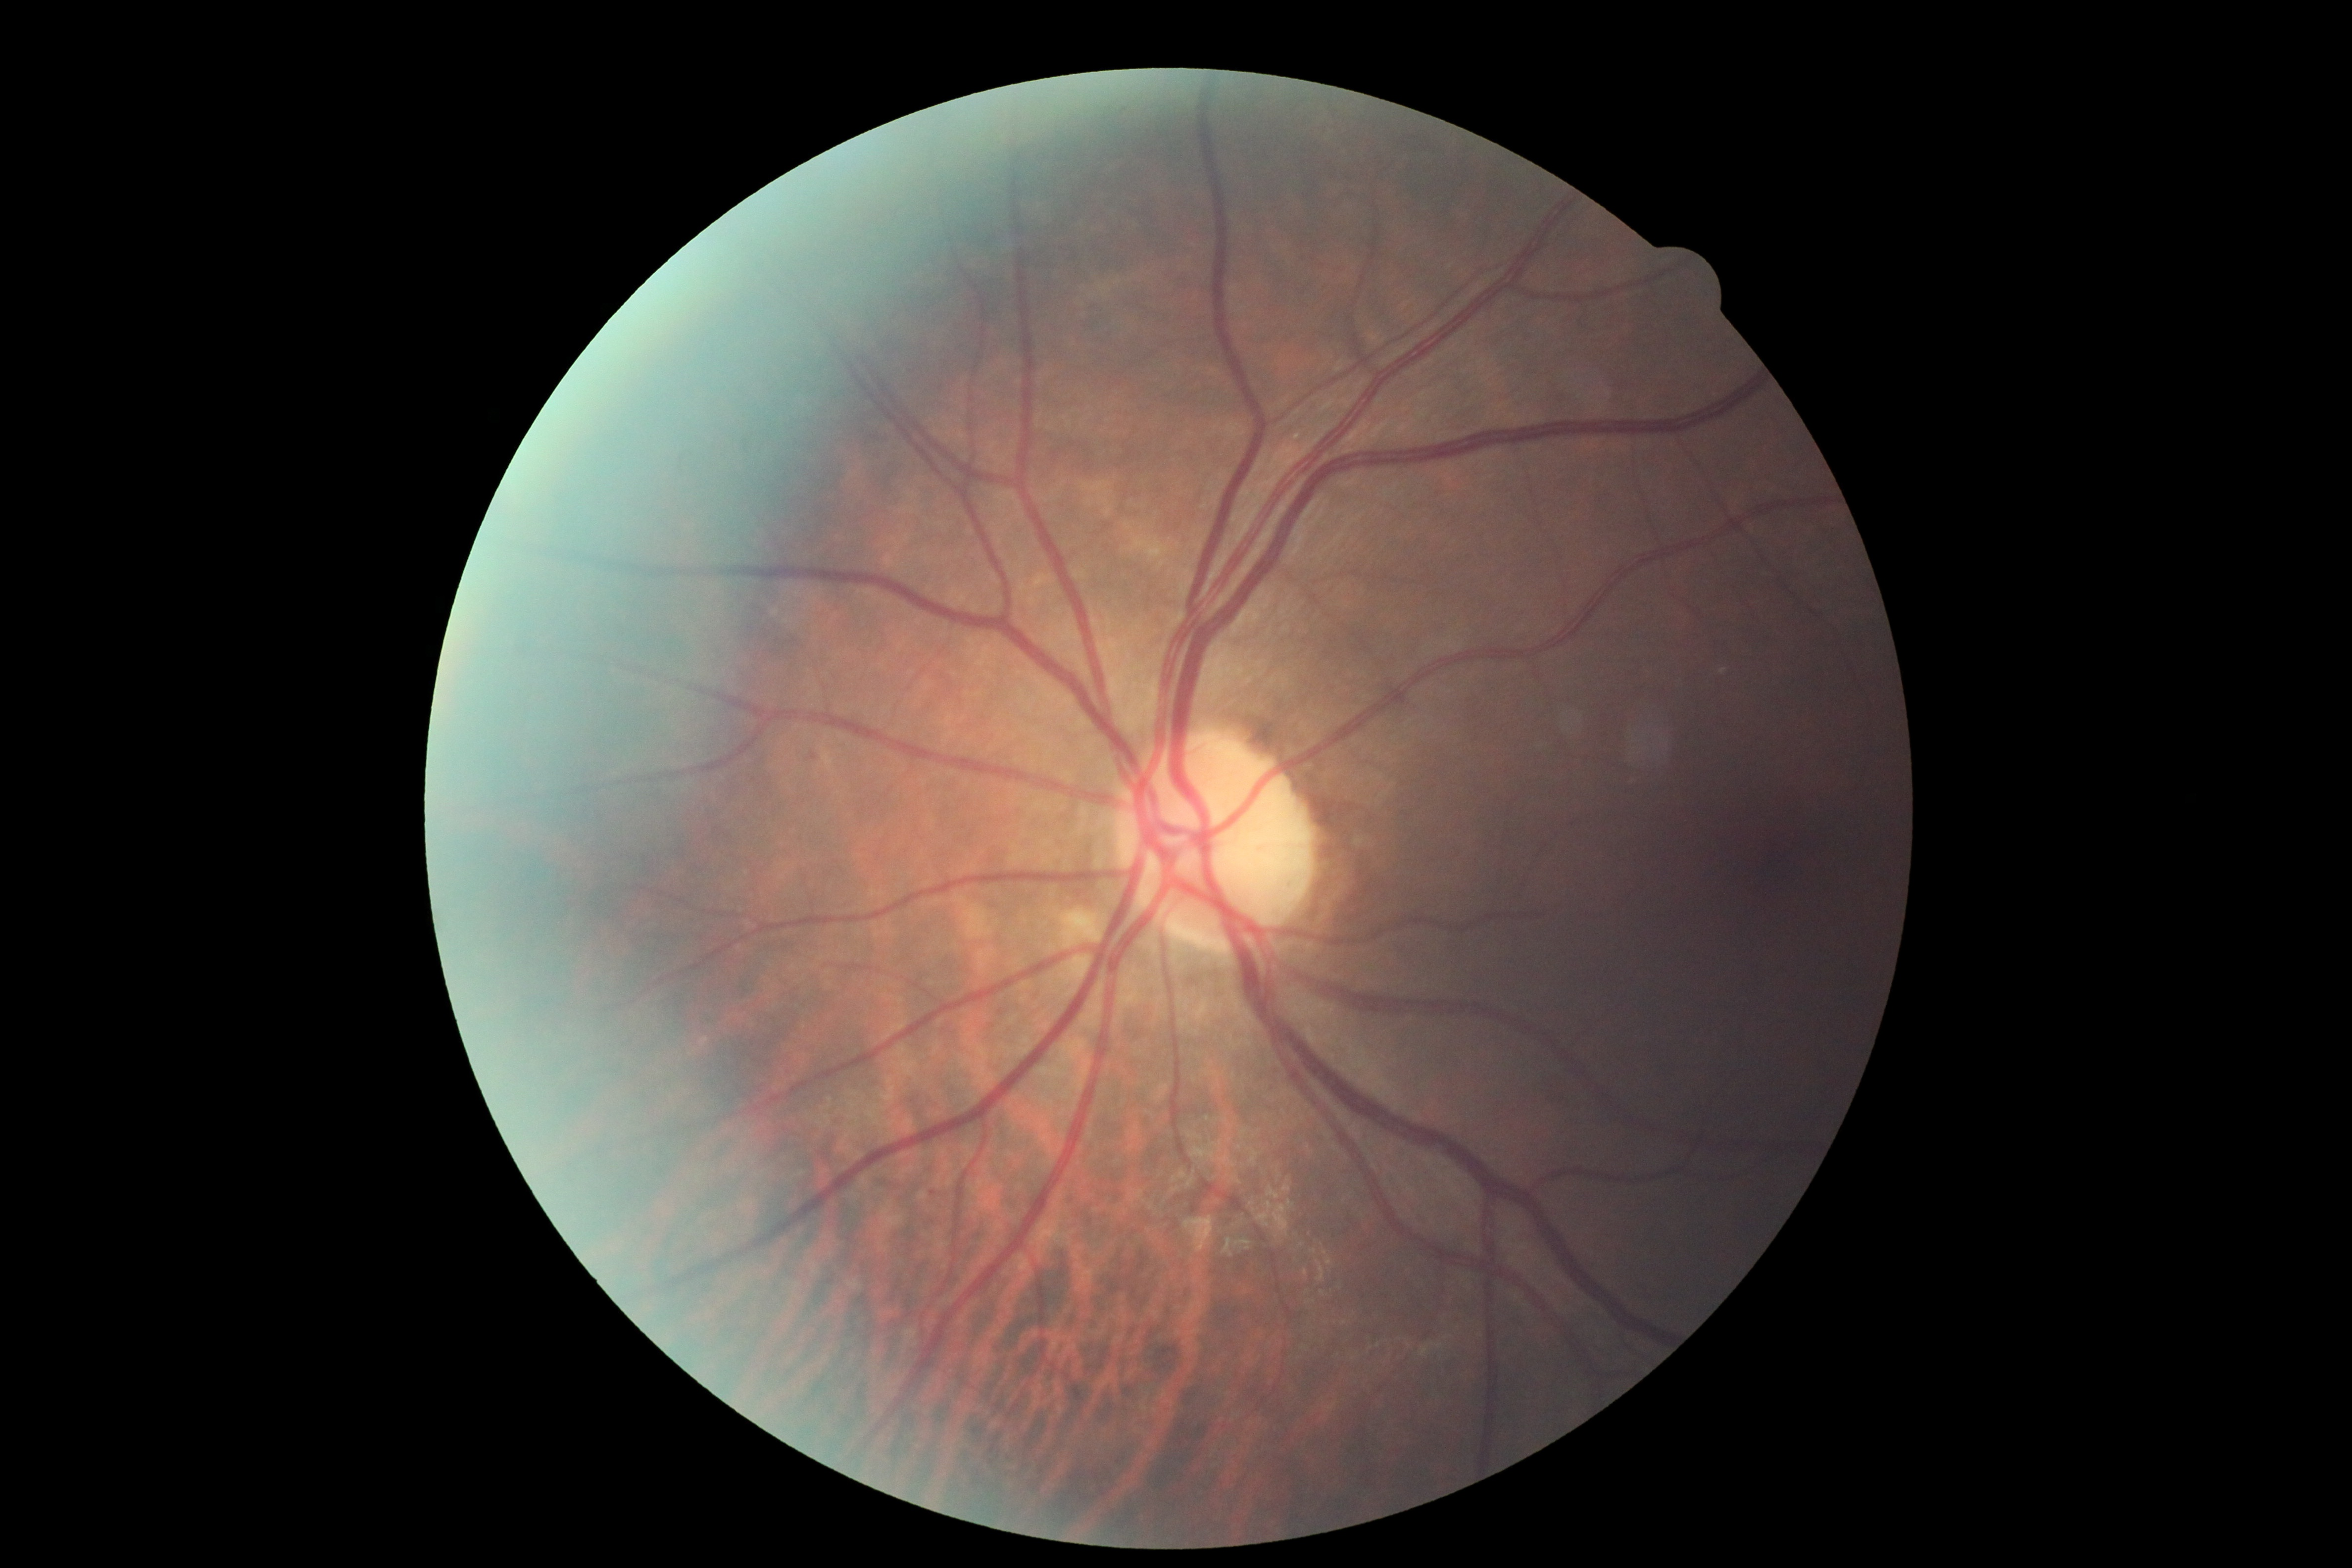
\includegraphics[scale=0.035]{images/0_Level_Example.jpeg}}
  \ \ \ \ 
\subfigure[Level 4 DR]{\label{new}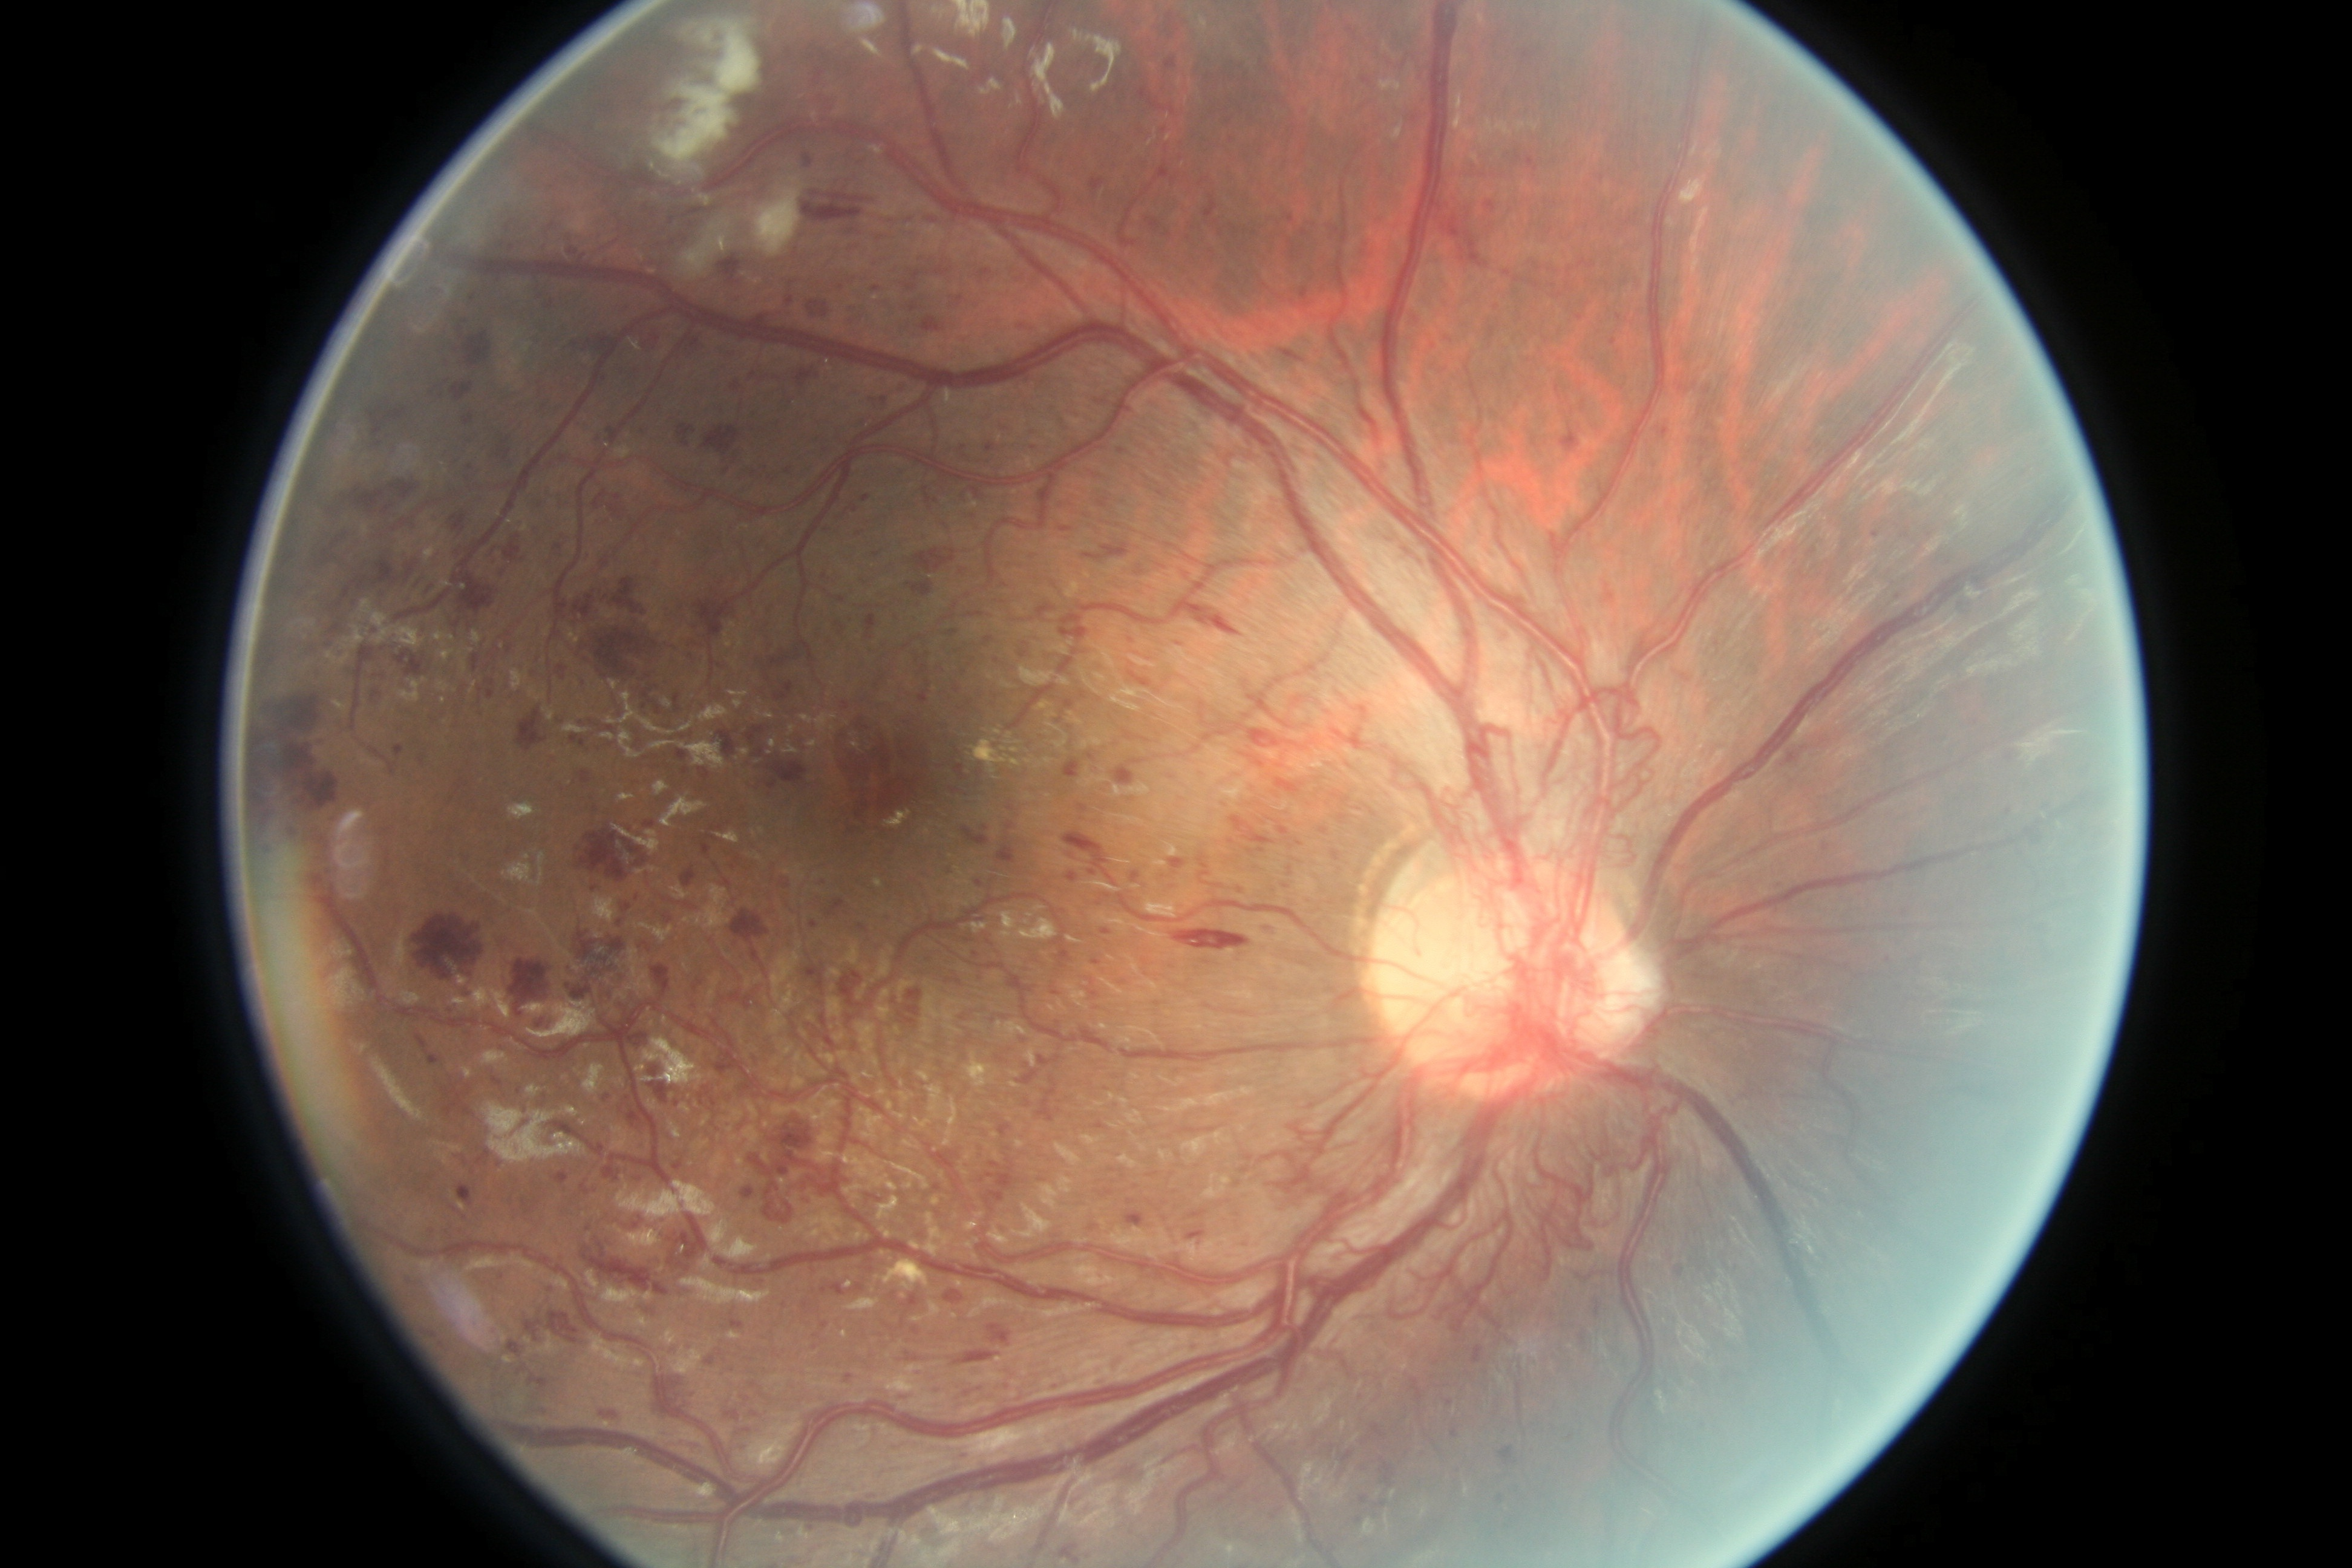
\includegraphics[scale=0.0425]{images/4_Level_Example.jpeg}}
\caption{Examples of level 0 and level 4 DR}
\label{marking_image}
\end{center}
\end{figure}

\subsection{The Kaggle Grand Challenge}

Kaggle has presented the automated DR diagnosis as open grand challenge. In doing so, Kaggle provided ~35 gigabytes of retinal scan data, over 35,000 images, thus each image is roughly 1.5 megabytes in size. To faciliate download and processing of the data set, Kaggle divided the image set into a training group, and a testing group, and the subsequently divided each group into smaller subsets to facilitate file transfer. All the results presented here and in subsequent discussions are based on the first training set of images.

It is noted that the aim of the current work is to understand ConvNN from a fundamental perspective, and not to actually create a competitive solution for the grand challenge. Due to the size of the reference data set, and the limitations imposed by Python in terms of loading elements into shared memory, it would be very difficult to create a code base that could compete directly with other implementations in CuDa, (a GPU-level system language), which is defacto favorite language for image processing.	

\section{Convolution Neural Networks}

ConvNN are a powerful machine learning technique that fall under the of general premise of deep learning. There are number of flavors of ConvNN, but the specific implementation presented here is one of the first implementations of the technique, the LeNet-5 \cite{LeNet}, and is especially adept at processing digital imaging.

The LeNet-5 consists of 3 primary component layers: the convolution layer, the pooling layer, the conventional fully connected layer \cite{deep}. 

\subsection{The Convolution Layer}

The convolution layer is the work horse of the ConvNN, at is what makes it such an indespensible tool for image processin. Mathematically, the concept of convolution is somewhat straightforward, and plays a key role in spectral methods and Fourier space treatments. In terms of digital imaging, convolution can be expressed as \cite{deep} the product of the pixel intensity of a given image with that of a kernel, and is stated as
\begin{equation}
H[m,n] * G[m,n] \, = \, \sum_{u=- \infty}^{\infty} \sum_{u=- \infty}^{\infty} H[u,v] G[m-u, n-v]
\end{equation}
This may seem somewhat convoluted at first, but consider that an image is an array of pixels, each with an intensity that ranges from 0 up to a given bit depth, (e.g. 255 for 8-bit images), than we can see that an image can be translated as matrix, where each element is a given pixel's image intensity. The concept is illustrated in \figref{matrix}
\begin{figure}[htbp]
\begin{center}
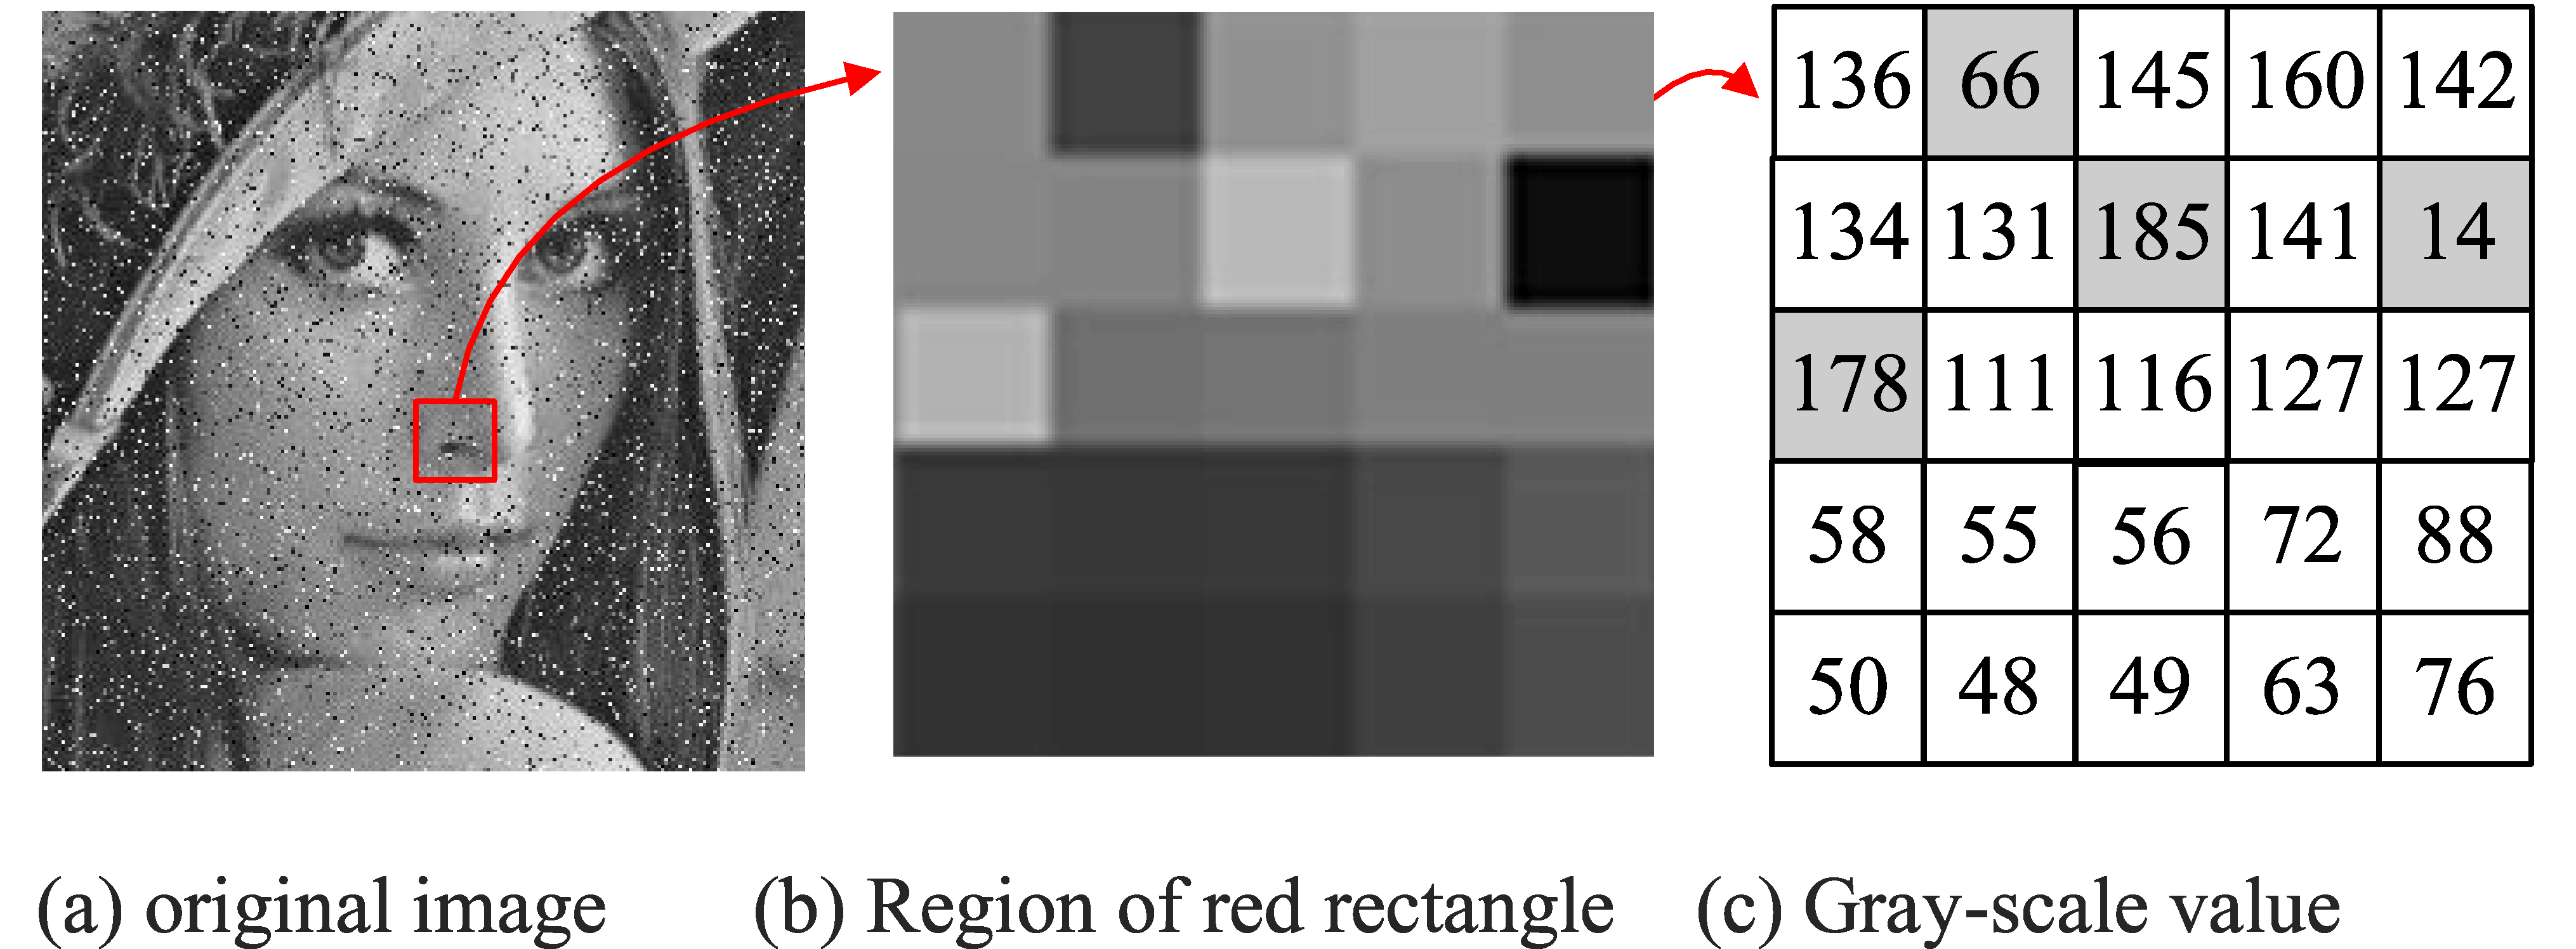
\includegraphics[scale=0.1]{images/lena.png}
\caption{Digital image as a matrix \cite{lena}}
\label{lena}
\end{center}
\end{figure}
A kernel, in the context of digital imaging, is itself a matrix of a prescribed dimension, such as 
\begin{equation}
H_{3 \times 3}^L \, = 
\begin{bmatrix}
  0 & 1  & 0 \\
  1 & -4 & 1 \\
  0 & 1  & 0
\end{bmatrix}
\label{lap_3x3}
\end{equation}
which is applied, via convolution across the matrix of the image.
\newpage
% \nocite{*}
\bibliographystyle{unsrt}
\bibliography{References}


\end{document}